\documentclass[aspectratio=169, compress]{beamer}

\usepackage[T1]{fontenc}
\usepackage[utf8]{inputenc}
\usepackage[english]{babel}
\usepackage{animate}
\usepackage{pgfplots}
\pgfplotsset{compat=newest}
\usepackage{booktabs}
\usepackage{siunitx}
\usepackage{subcaption}
\usepackage{tikz}
\usepackage{tikz-3dplot}
\usepackage{bm}
\usetikzlibrary{calc}
\usepackage{tikzpagenodes}
\usepackage{amsmath,amssymb,amsfonts, stmaryrd}
\usepackage{pgfplots}
\usetikzlibrary{shapes,arrows,decorations.pathmorphing,backgrounds,positioning,fit,matrix}
\usepackage{mathtools} %Fixes/improves amsmath
\usepackage{lipsum}
\pgfplotsset{compat=1.8}
\usepackage{graphics} % for pdf, bitmapped graphics files
\usepackage{epsfig} % for postscript graphics files
\usetikzlibrary{spy}
% Latin Modern
\usepackage{lmodern}
% Verdana font type
%\usepackage{verdana}
% Helvetica
%\usepackage{helvet}
% Times (text and math)
%\usepackage{newtx, newtxmath}
% Nice font combination
%\usepackage{mathptmx} % math
%\usepackage{sourcesanspro} % sans-serif
\usepackage{charter} % serif

\usetheme[department=space]{DTU}
\useoutertheme[subsection=false]{miniframes}
%\useoutertheme{split}
\setbeamercovered{transparent}
%\setcounter{currentslide}{\the\beamer@slideinframe}

\title{Photogrammetry (30540)}
\subtitle{Feature Detection, Matching, RANSAC \& Bundle Adjustment}
\author{\textbf{Instructor}: Daniel Olesen$^1$ \\
	\textbf{TA}: Xiao Hu$^2$}
\institute{$^1$: Assistant Professor, Dept. of Geodesy\\ $2$: PhD student}
\date{\today}

\newcommand{\tabitem}{{\color{dtured}$\bullet$} }

\begin{document}
	\frame{
		\maketitle
	}
	
	\frame{
		\frametitle{Today's Lecture}
		\tableofcontents
	}
	
	
	
	\section{Image Feature}
	\subsection{Feature Detection}
	\frame{
		\frametitle{Feature Definition} 
		Features are recognizable structures of elements in the environment: 
		\begin{itemize}
		\item low-level features (geometric primitives): lines, \textcolor{red}{points}, blobs, circles or polygons.
		\item high-level features (sematic objects): doors, tables, or trash cans.
		\end{itemize}
		Features serve as more compact and robust description of the environment.

		\begin{figure}
			\centering
			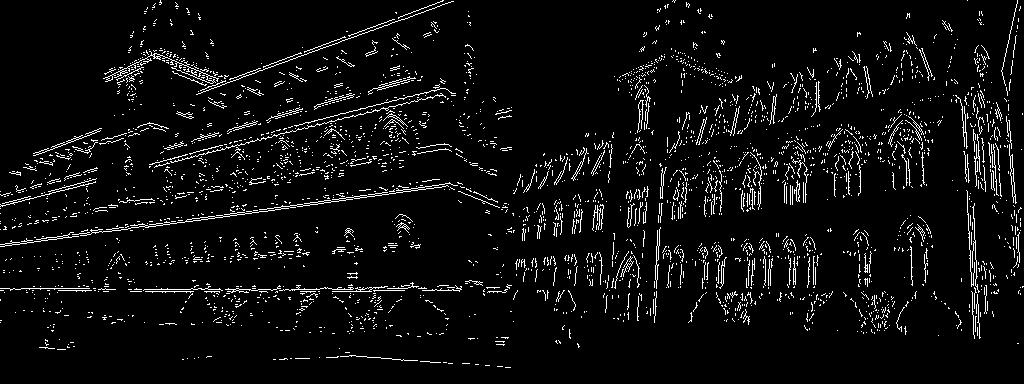
\includegraphics[width=0.6\textwidth]{figures/edge.jpg}
			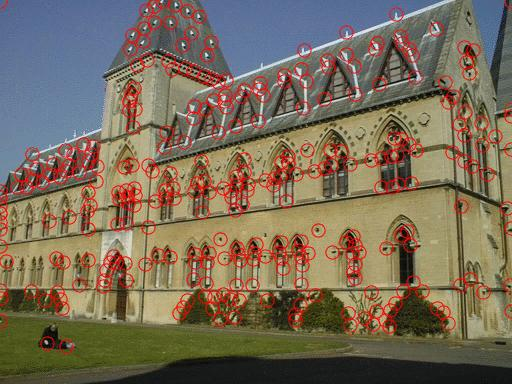
\includegraphics[width=0.3\textwidth]{figures/xiaohan_harris.jpg}
		\end{figure}
	}

	\frame{
		\frametitle{Feature Detection:  Keypoint Detectors}
		Properties of the ideal feature detector:
		\begin{itemize}
			\item Repeatability: can be redetected regardless view/illumination changes: \textcolor{red}{rotation, scale (zoom), and illumination invariant}.
			\item Distinctiveness: easy to distinguish and match.
			\item Localization accuracy.
			\item Computational efficiency.
		\end{itemize}
		Two major groups:
		\begin{enumerate}
			\item Corner detectors: Harris\cite{c2}, FAST\cite{c3}, etc.
			\item Blob feature detectors: SIFT\cite{c4}, etc.
		\end{enumerate}
	}

	\frame{
		\frametitle{Corner detector: Harris}
		A corner in an image can be defined as the intersection of two or more edges.
		\begin{figure}
			\centering
			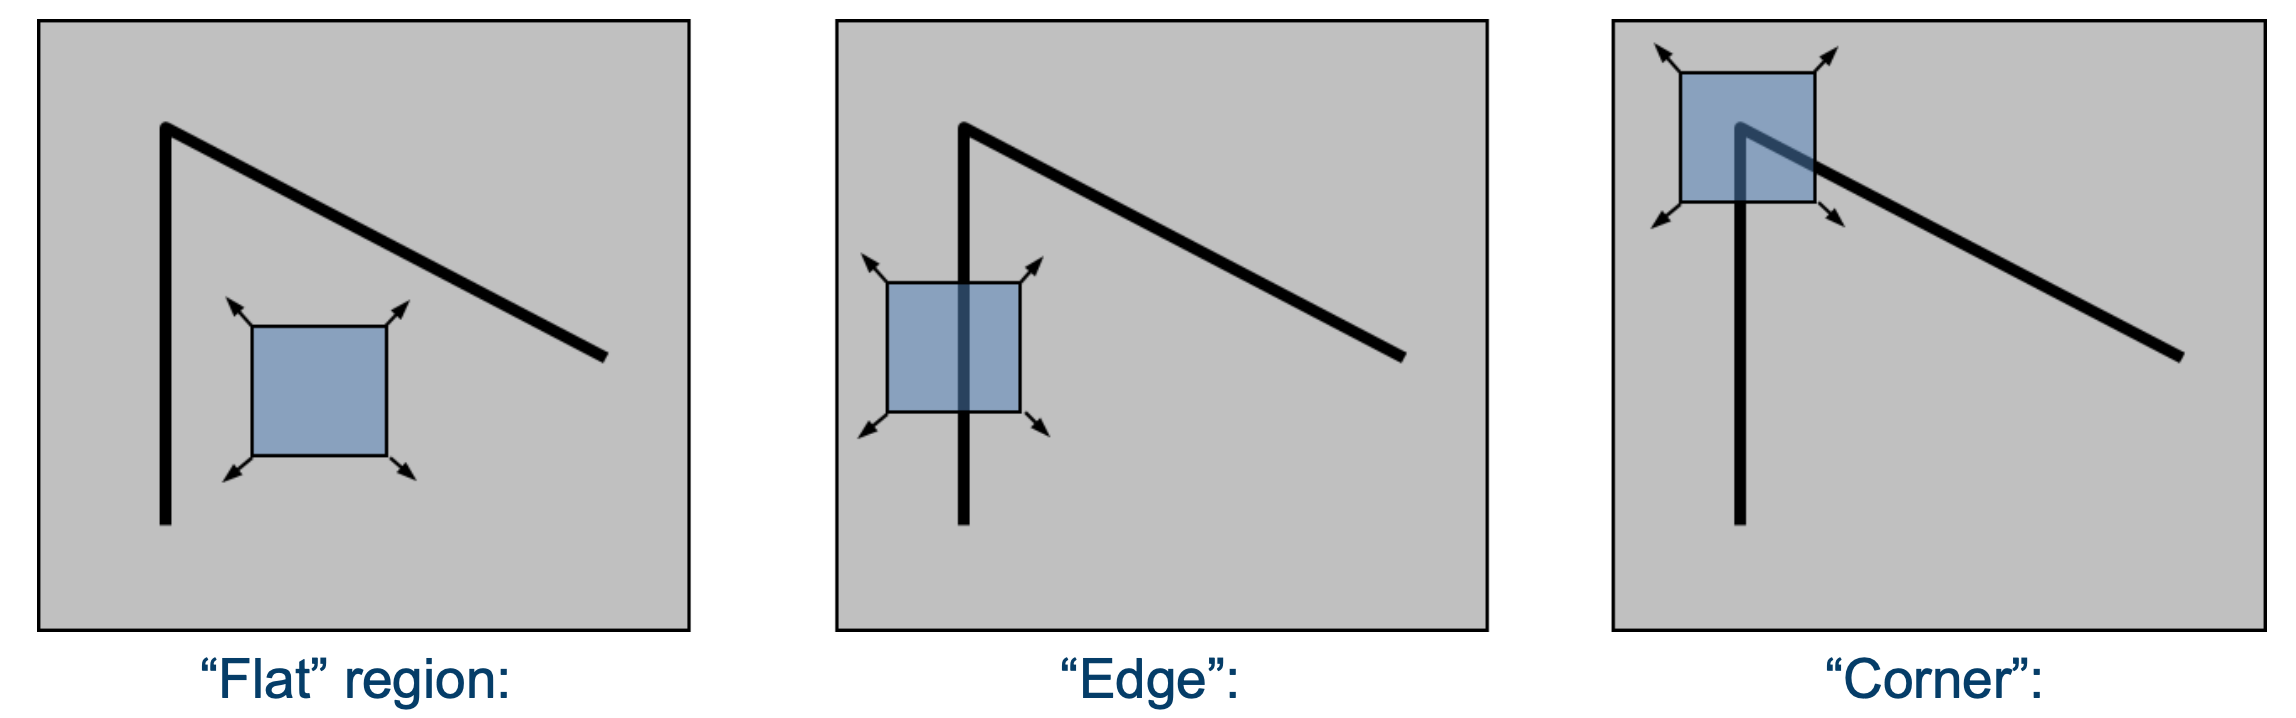
\includegraphics[width=0.8\textwidth]{figures/corner1.png}
			\caption{Illustration of Corner keypoint\cite{c5}.}
		\end{figure}
		What should be inside the sliding window $\to$ the partial derivatives of the Sum of
Squared Differences (SSD).
		}
	\frame{
		\frametitle{Corner detector: Harris}
			SSD:
			$$\text{SSD}(x,y)=\sum_{u}\sum_{v}{(I(u,v)-I(u+x,v+y))^2}$$
			$I(u+x,v+y)$ can be approximated by a first-order Taylor expansion using partial derivatives $I_x$ and $I_y$:
			$$I(u+x,v+y)\approx I(u,v)+I_x(u,v)x+I_y(u,v)y$$
			This produces the approximation of SSD:
			$$
			\text{SSD}(x,y)\approx \sum_{u}\sum_{v} (I_x(u,v)x+I_y(u,v)y)^2 = [x,y]\underbrace{\left(\sum_{u}\sum_{v}\left[\begin{matrix}
			I_x^2 & I_xI_y \\
			 I_xI_y &  I_y^2
			\end{matrix}\right]\right)}_{\mathbf{M}}[x,y]^T
			$$
			The Harris detector analyses the eigenvalues of to verify whether currecnt point is a corner or not.
		}
	\frame{
		\frametitle{Corner detector: Harris}
			\begin{columns}
			\column[c]{.5\textwidth}
			\begin{figure}
				\centering
				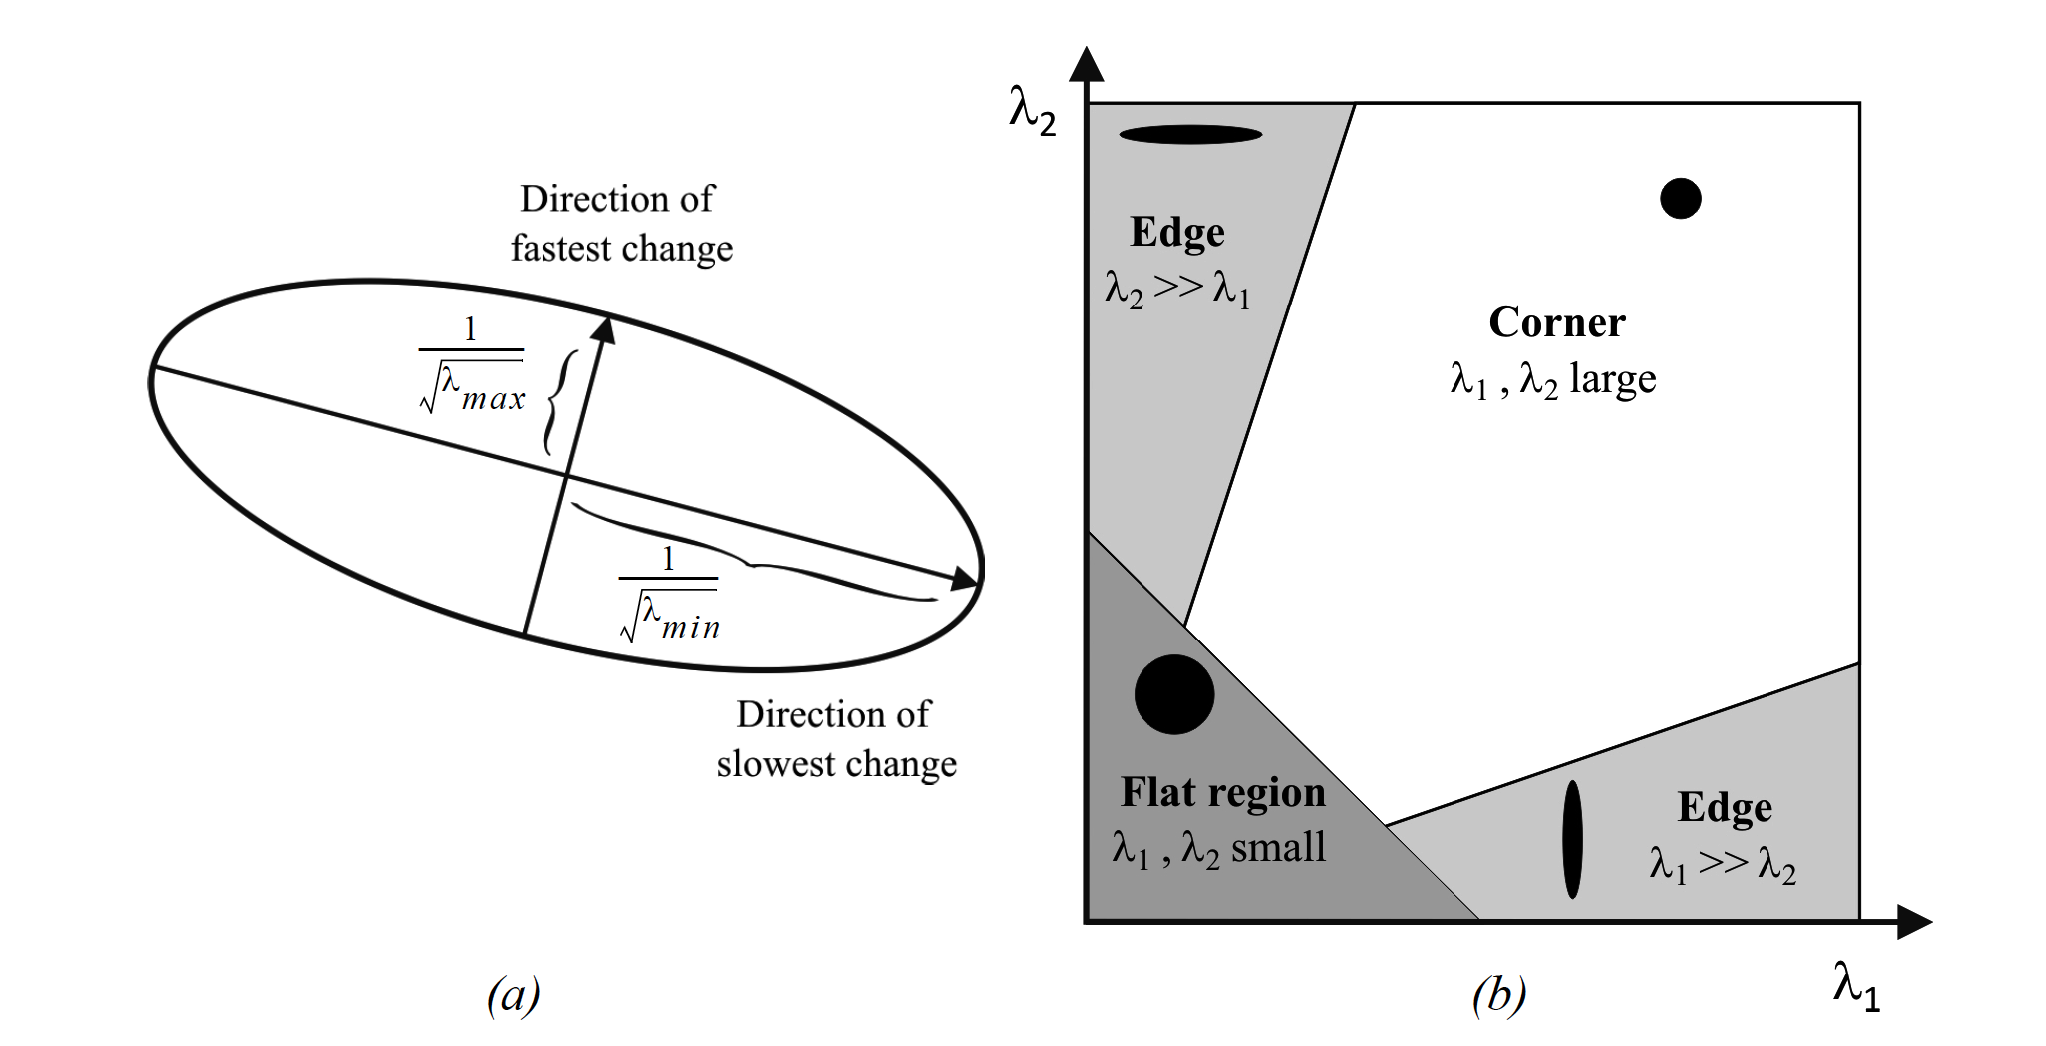
\includegraphics[width=1\textwidth]{figures/corner2.png}
				\caption{The classification of corner and edges according to Harris and
Stephens\cite{c6}.}
			\end{figure}
			\column[c]{.5\textwidth}
			For easy computation, the following “cornerness function” is actually used:
			$$
			C = \lambda_1\lambda_2-k(\lambda_1+\lambda_2)^2=\text{det}(\mathbf{M})-k\cdot \text{trace}(\mathbf{M})
			$$
			Harris corner point is then found as the local maximum by using nonmaxima suppression. 
			
			In conclusion, Harris keypoint is \textcolor{red}{rotation/translation invariant, but not scale invariant.}
			\end{columns}
		}
	\frame{
		\frametitle{Corner detector: Harris}
		Let's see an example:
		\begin{figure}
			\centering
			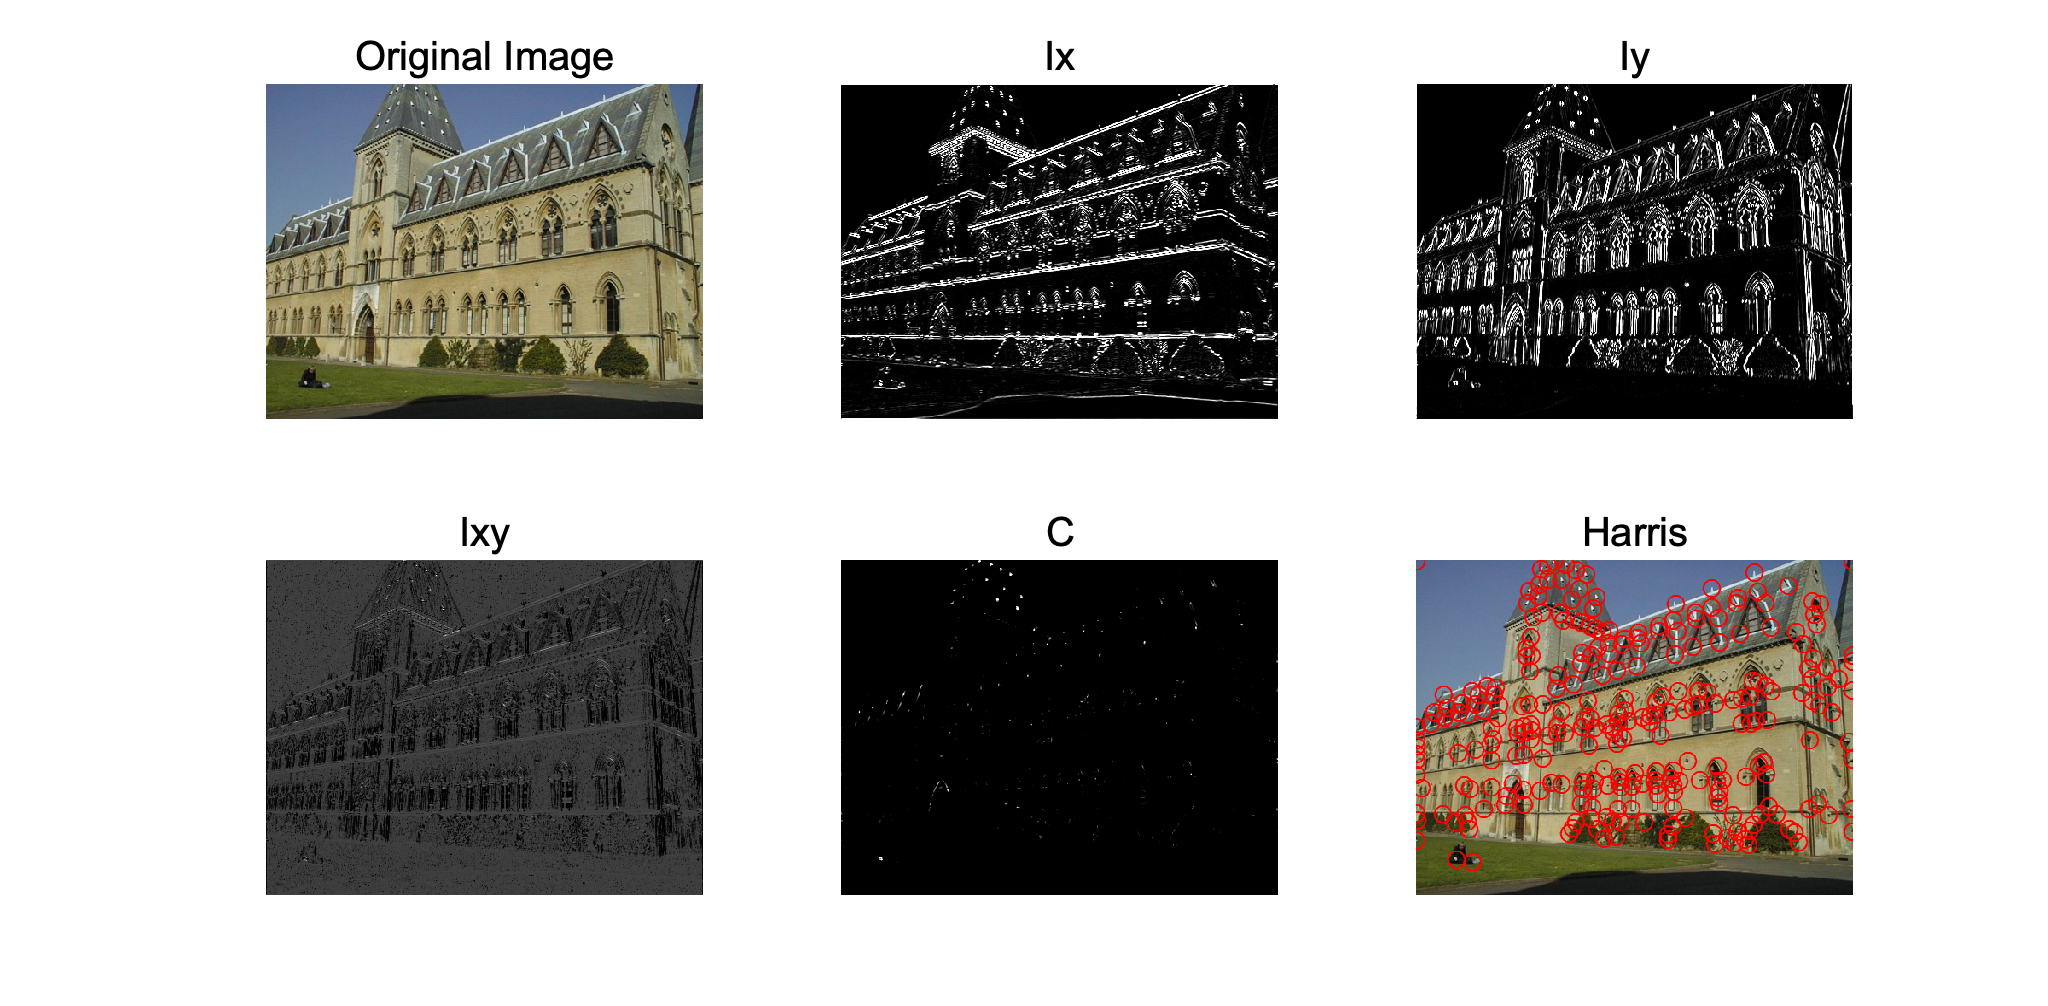
\includegraphics[width=1\textwidth]{figures/corner3.png}
		\end{figure}
	}
	\frame{
		\frametitle{Other corner detectors}
		\begin{itemize}
			\item Shi-Tomasi corner detector or GFTT: use $min(\lambda_1,\lambda_2)$.
			\item FAST: compares $16$ pixels on a circle around the candidate corner. Not rotation invariant, but super fast.
		\end{itemize}
		\begin{figure}
			\centering
			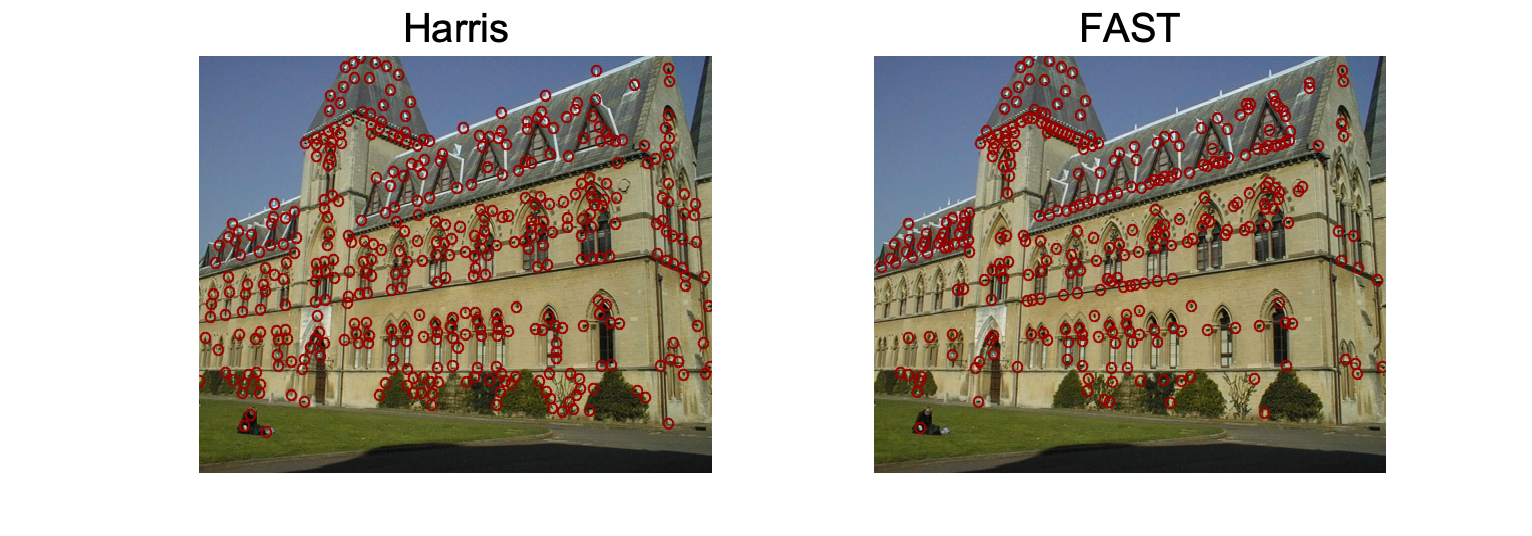
\includegraphics[width=0.8\textwidth]{figures/corner4.png}
			\caption{Comparison of Harris and FAST.}
		\end{figure}
	}
	
	
	\frame{
		\frametitle{Blob Detectors}
		Blob is an pattern which differs from its immediate neighborhood in terms of
		intensity, color, and texture. 
		
		Scale Invariant Feature Transform(SIFT)\cite{c4} is the most popular blob feature detector, which is widly used in mapping and navigation, etc thanks to its robustness to rotation and small changes of illumination, scale.
		
		Main steps of the SIFT algorithm:
		\begin{itemize}
			\item find keypoint location and scale.
			\item find dominant orientation.
			\item generate keypoint descriptor.
		\end{itemize}
		So, SIFT $=$ keypoint $+$ descriptor.
	}

	\frame{
		\frametitle{Find keypoint location and scale}
			\begin{columns}
			\column[c]{.4\textwidth}
			\begin{itemize}
				\item Build up scale space.
				\item Compute Difference of Gaussian (DoG).
				\item Find local extrema across adjacent scales, then additional substeps like elimination points on edges or in very flat regions, interpolation of feature's location.
			\end{itemize}
			\column[c]{.6\textwidth}
			\begin{figure}
			\centering
			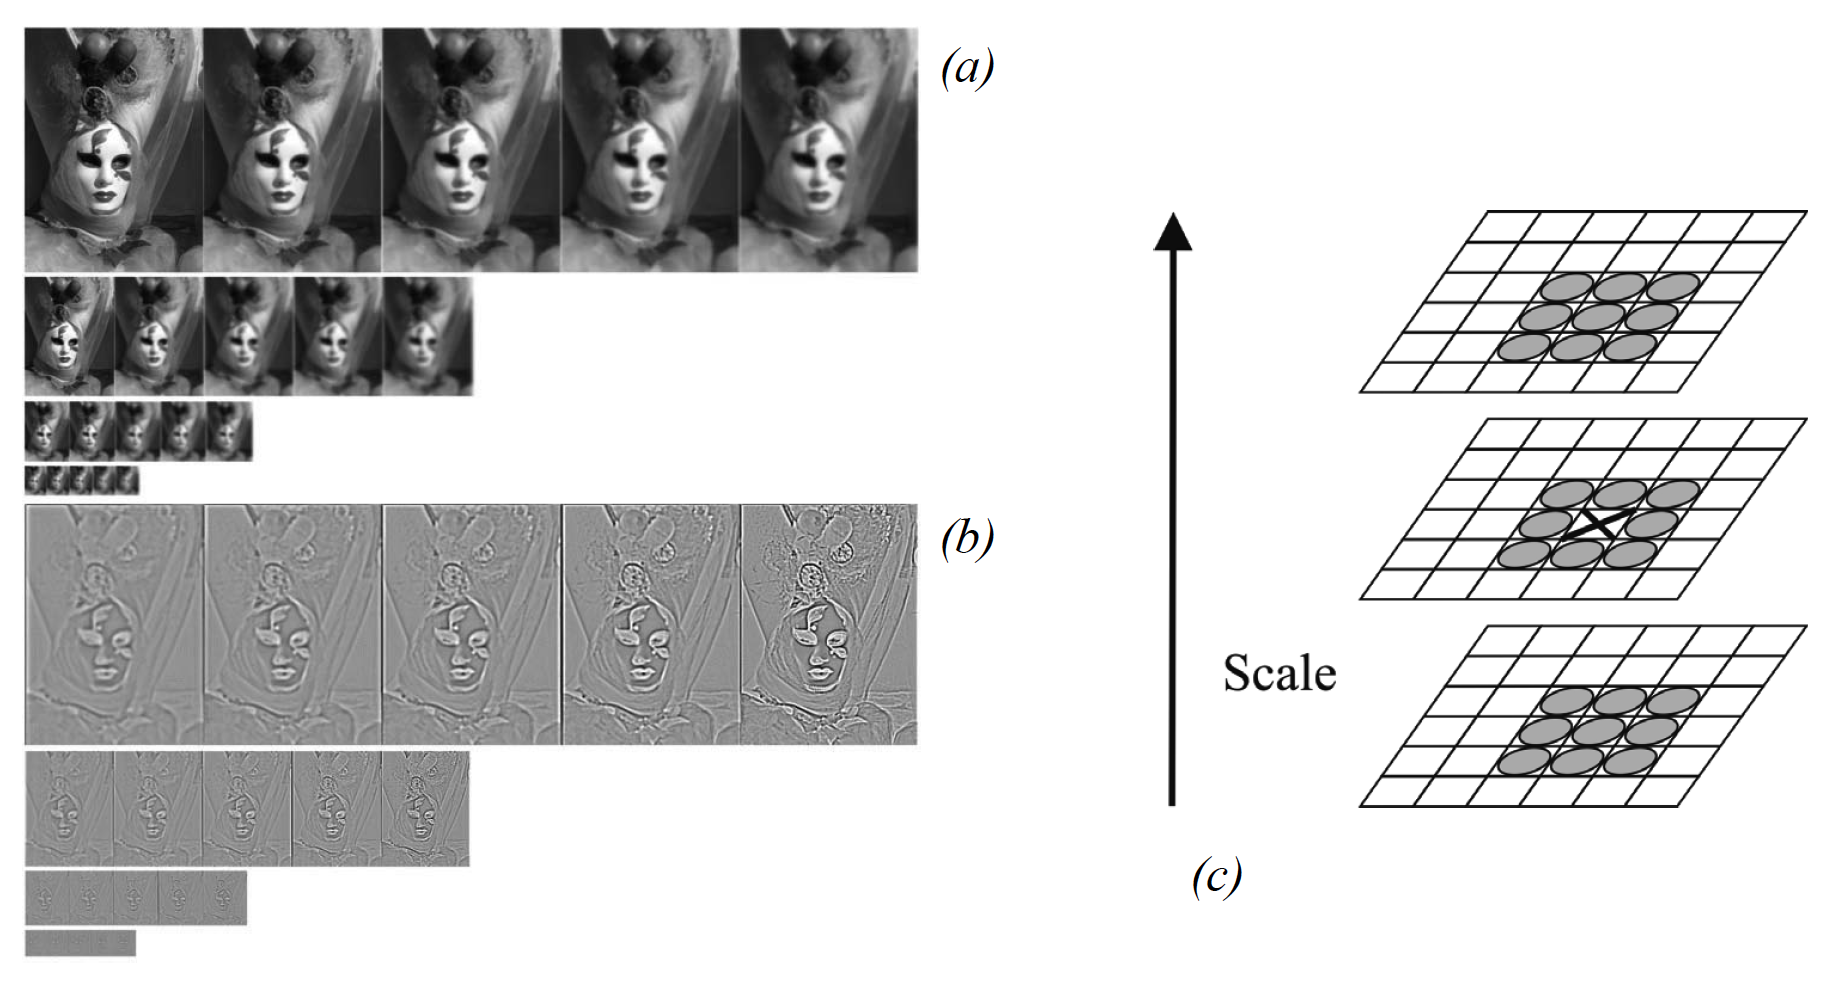
\includegraphics[width=1\textwidth]{figures/sift1.png}
			\caption{Scale space and DoG images.\cite{c6}.}
			\end{figure}
		\end{columns}
	}

	\frame{
	\frametitle{Find dominant orientation.}
	\begin{columns}
		\column[c]{.5\textwidth}
		The dominant orientation is used to make the descriptor rotation invariant.
		\begin{itemize}
			\item Compute the gradient magnitude and orientation in the image with closet scale.
			\item Build a gradient magnitude weighted histogram of orientations within a Gaussian-weighted circular window. 
			\item Find the peaks as the dominant orientation. If the second peak is within 80\% of the first peak, an additional keypoint is created.
		\end{itemize}
		\column[c]{.5\textwidth}
		\begin{figure}
			\centering
			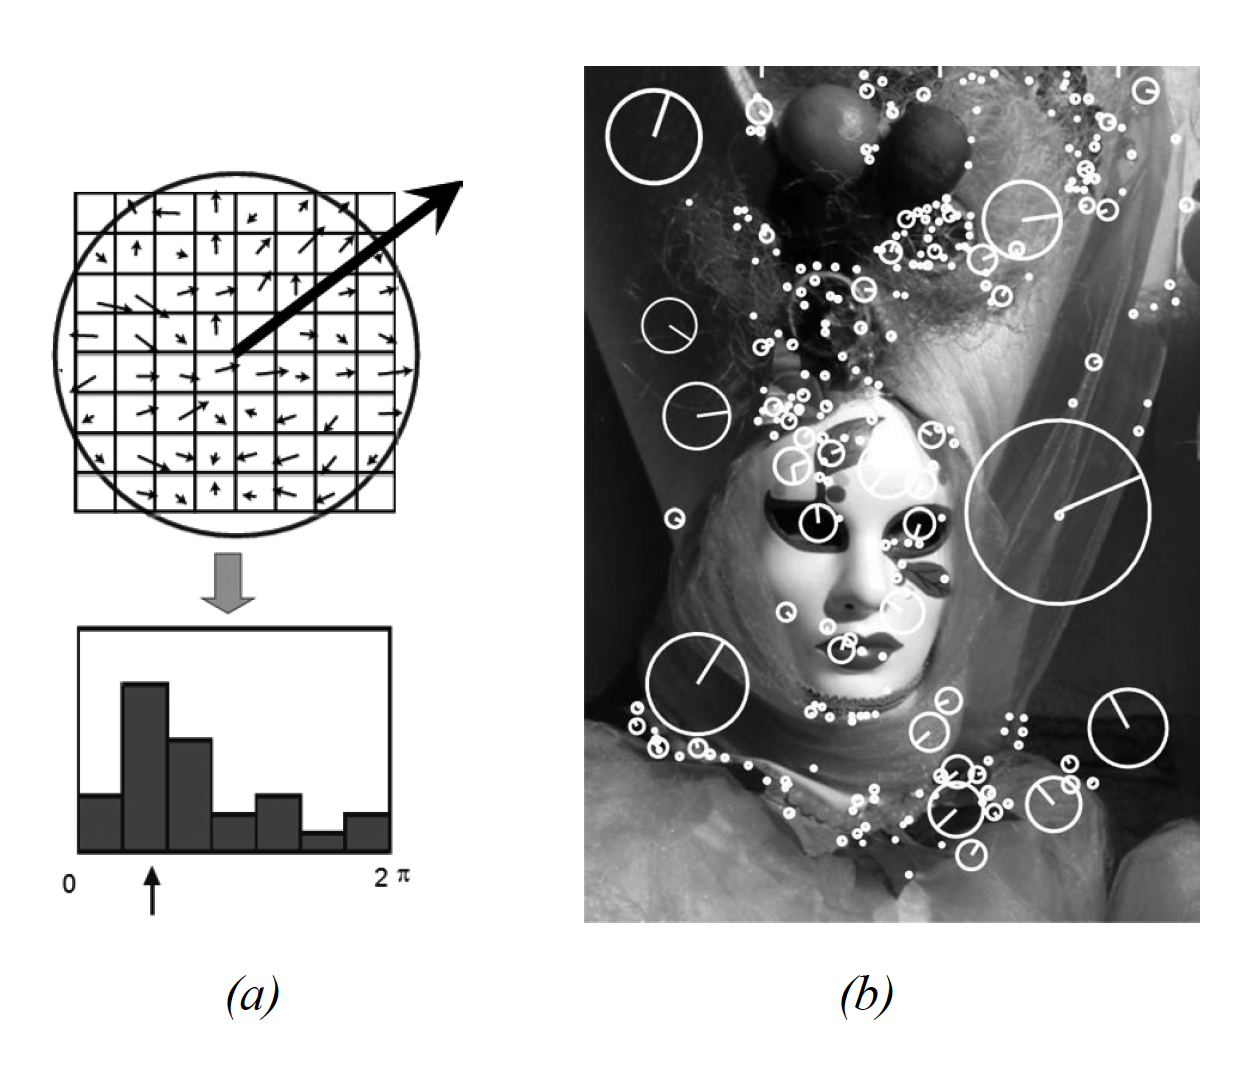
\includegraphics[width=0.9\textwidth]{figures/sift2.png}
			\caption{Histogram of orientation and examples of SIFT features with different scales and dominant orientations\cite{c6}.}
		\end{figure}
	\end{columns}
	}

	\frame{
	\frametitle{Generate feature descriptor}
	\begin{columns}
	\column[c]{.5\textwidth}
	\begin{itemize}
		\item Rotate the gradient orientations relative to the keypoint dominant orientation.
		\item The Gaussian window  is then divided into $4\times 4$ regions. A second histogram of gradient with eight orientation bins is computed within each region.
		\item The descriptor is built by flattening the orientation histograms and concatenating them to form a $4\times 4 \times 8=128$ vector.
		\item Normalization, clipping and renormalization for illumination invariant.
	\end{itemize}
	
	\column[c]{.5\textwidth}
	\begin{figure}
		\centering
		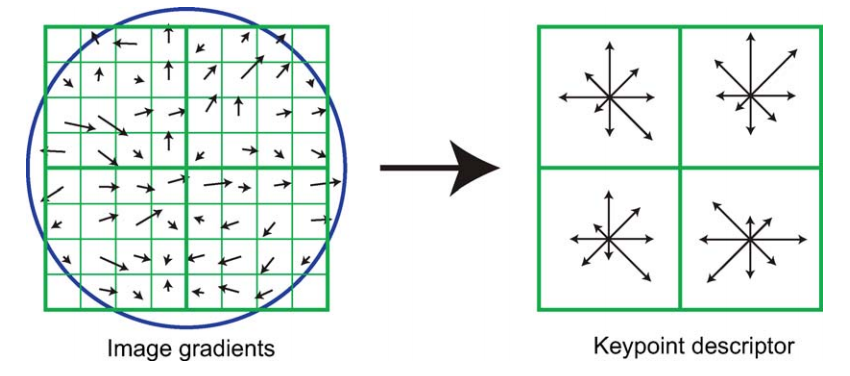
\includegraphics[width=0.9\textwidth]{figures/sift3.png}
		\caption{Gaussian circular windown and $4\times 4$ regions with histograms of gradient with $8$ bins\cite{c4}.}
	\end{figure}
\end{columns}
	}	

	\subsection{Feature Description}
	\frame{
	\frametitle{Descriptor}
	\begin{columns}
		\column[c]{.5\textwidth}
		Keypoint needs a descriptor in order to perform feature matching:
		\begin{itemize}
			\item Histogram of Gradients (HoG) descriptors, like SIFT.
			\item Binary descriptors, like BRIEF\cite{c8}.
		\end{itemize}
			\column[c]{.5\textwidth}
		\begin{figure}
			\centering
			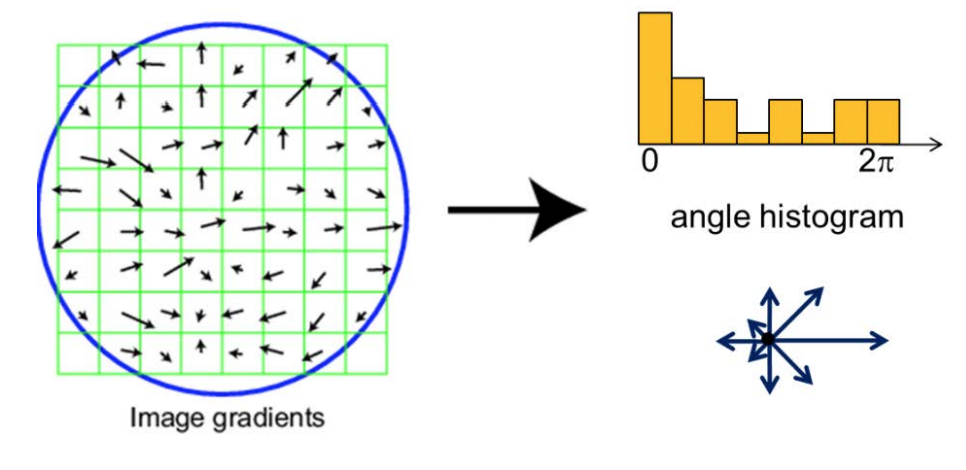
\includegraphics[scale=0.35]{figures/desp1.png} \\
			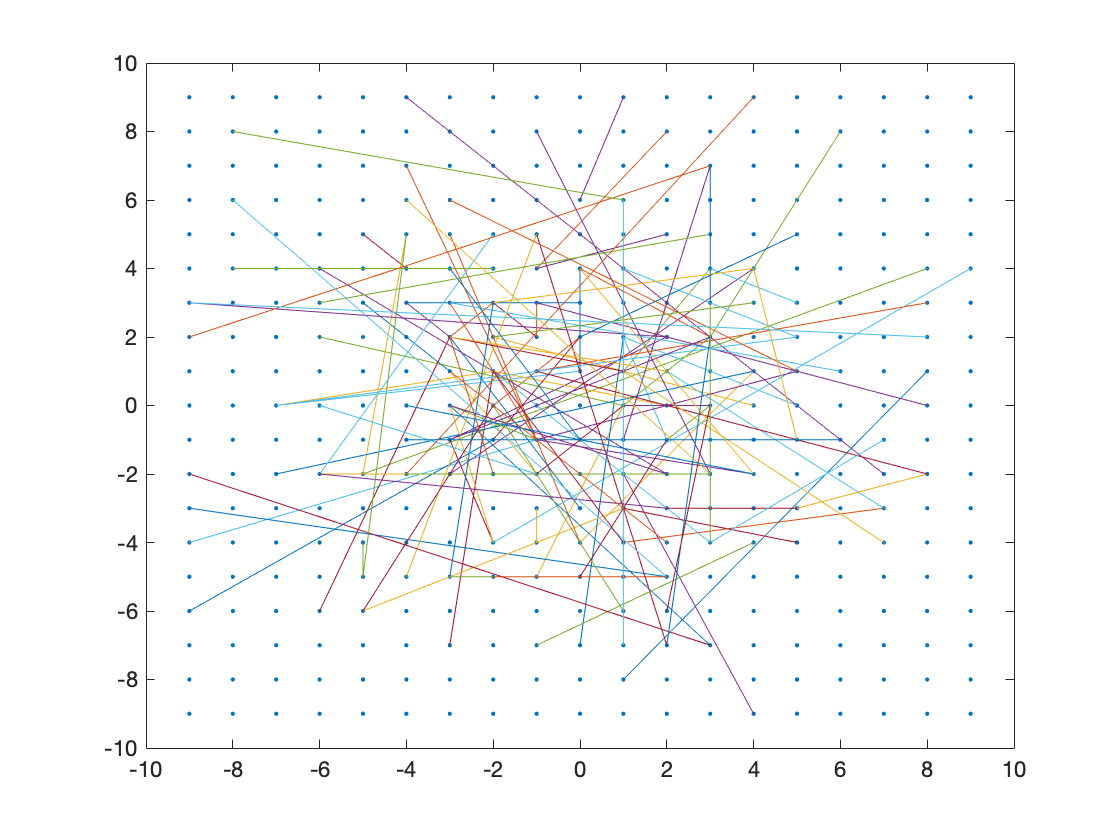
\includegraphics[scale=0.13]{figures/desp2.png}
			\caption{Histogram of Gradients (HoG) descriptor and Binary descriptor.}
		\end{figure}
		\end{columns}
	}		

	\subsection{Summary on Features}
	\frame{
		\frametitle{Summary}
		\begin{figure}
			\centering
			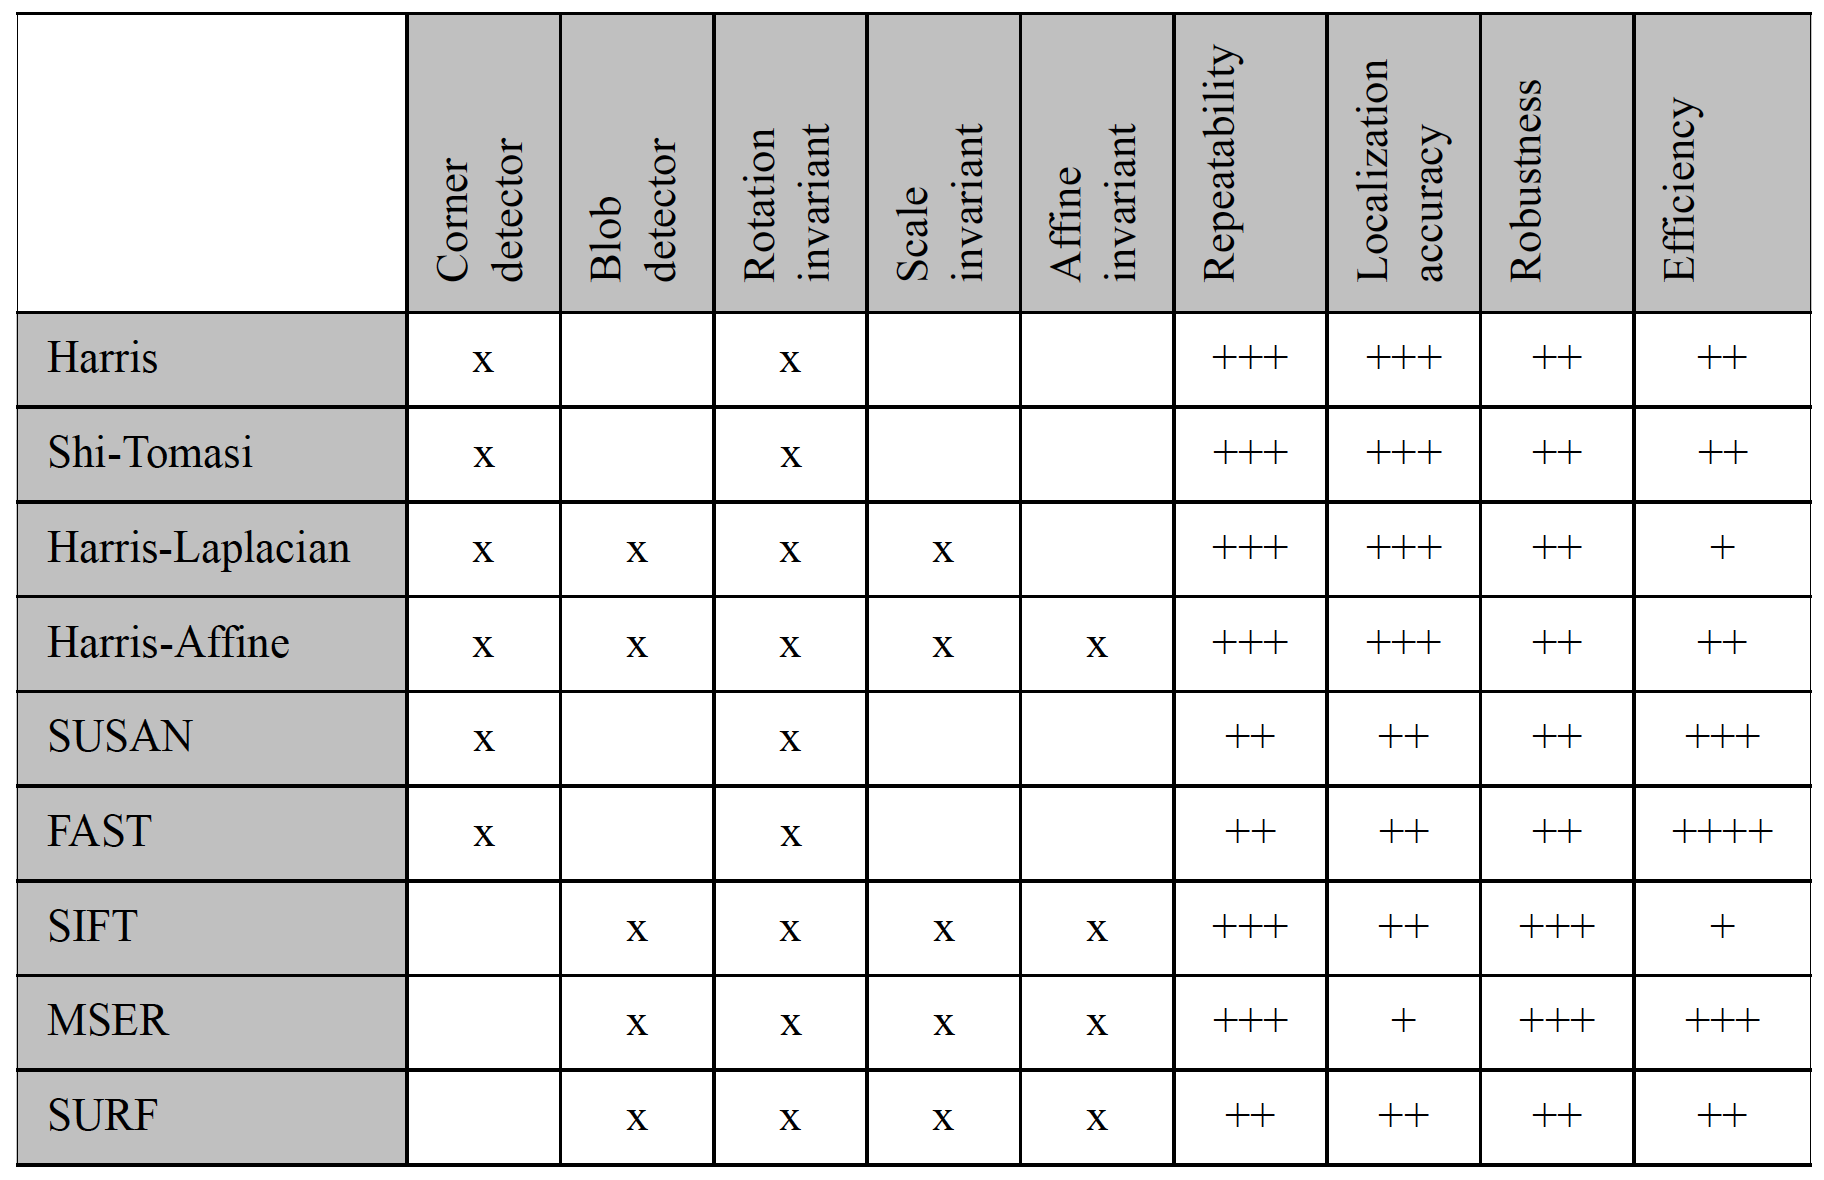
\includegraphics[width=0.7\textwidth]{figures/desp3.png}
			\caption{Comparison of feature detectors: properties and performance\cite{c6}.}
		\end{figure}
	}
	\frame{
		\frametitle{Summary}
		\begin{itemize}
			\item SIFT is the most used feature in modern Photogrammetry.
			\item ORB and Harris are often used in visual odometry, VSLAM, tracking.
			\item Hand-crafted features are now challenged by deep learning based features, e.g. LIFT\cite{c9} V.S. SIFT. More learning based features are emerging. However, their usages in Photogrammetry are still in development (could be an research interest).
		\end{itemize}
		\begin{figure}
			\centering
			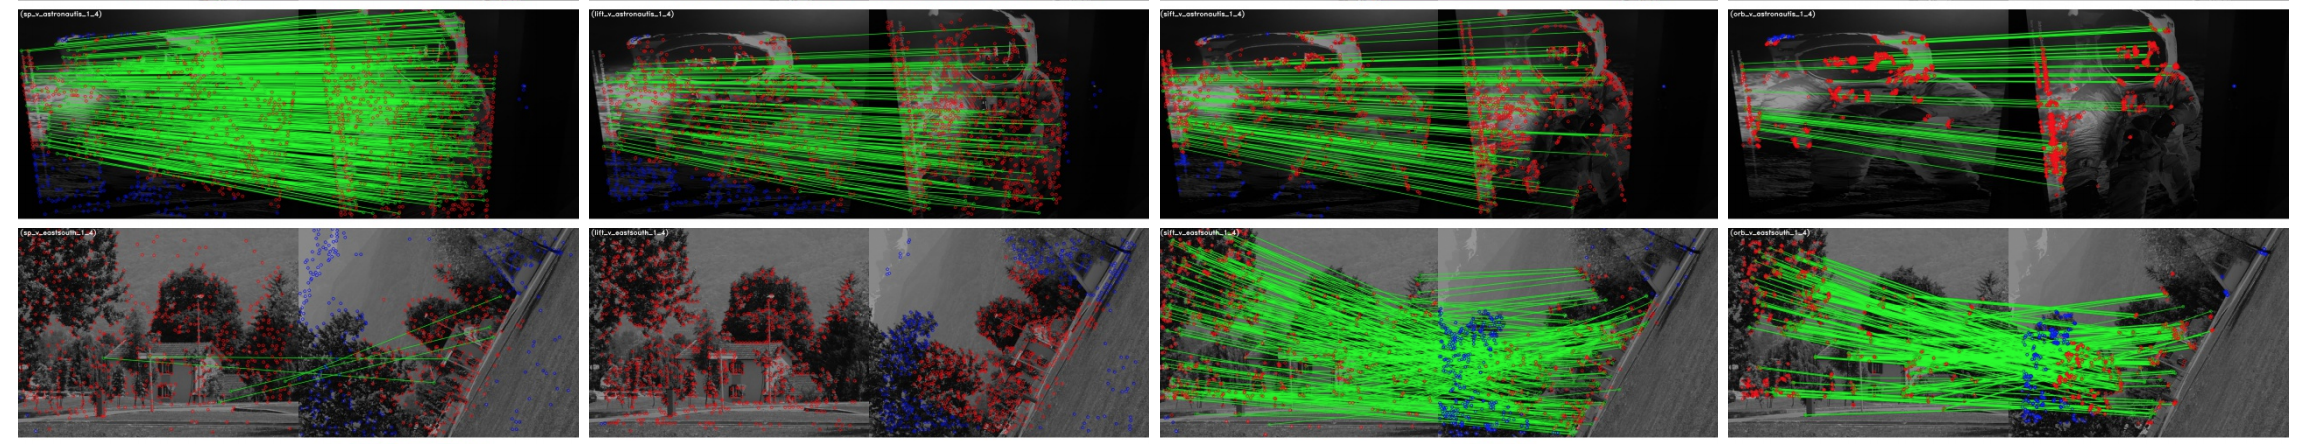
\includegraphics[width=1\textwidth]{figures/lift2.png}
			\caption{Comparison of Superpoint, LIFT, SIFT, and ORB.\cite{c10}.}
		\end{figure}
	}
	\section{Feature Matching}
	{
		\subsection{Principles}	
		\frame{
			\frametitle{Principles}
			\begin{columns}
				\column[c]{.5\textwidth}
				\begin{figure}
					\centering
					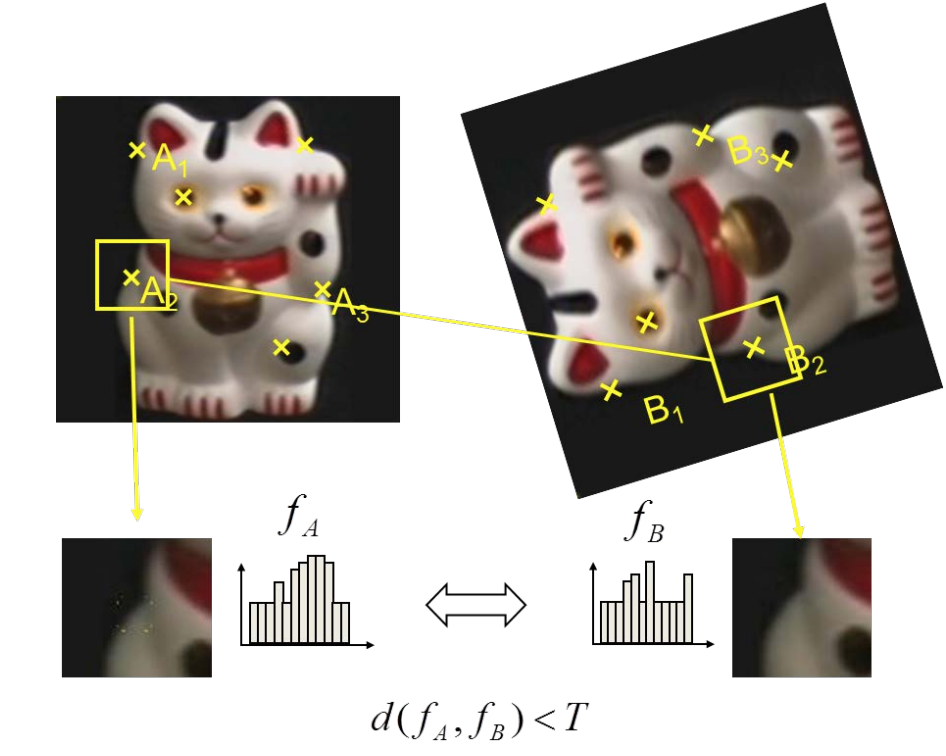
\includegraphics[width=1\textwidth]{figures/matching1.png}
					\caption{Principle of feature matching\cite{c11}.}
				\end{figure}
				\column[c]{.5\textwidth}
				Different distance functions for comparing the similarity of two descriptors:
				\begin{itemize}
					\item $\text{L}_2$ distance, for descriptors with floating value (SIFT):
					$$
					d(f_a,f_b) = \sum_i||(f_a(i)-f_b(i))||_2
					$$
					\item Hamming distance, for descriptors with binary value (BRIEF):
					$$
					d(f_a,f_b) = \sum_i\text{XOR}(f_a(i),f_b(i))
					$$
					\item others: $\text{L}_1$ distance, etc.
				\end{itemize}
			\end{columns}
		}	
	\subsection{Matching strategy}	
	\frame{
	\frametitle{Matching strategy}
		\begin{columns}
			\column[c]{.5\textwidth}
			Comparing strategy:
			\begin{itemize}
				\item Brute-force matching: for $a$ in image $1$, compare all $b$ in image $2$.
				\item Kd tree: binary search in Kd tree.
			\end{itemize}
			Selecting strategy:
			\begin{itemize}
				\item Take the nearest.
				\item Take the nearest with the distance below a threshold.
				\item Take the two closest and perform ratio test:
						$$
						\frac{d_{closet}}{d_{second\_closet}} < \tau
						$$
						$\tau$ is usually set to $0.7$.
				\item Cross-check: $f_b$ is the best match for $f_a$ in image $2$ and $f_a$ is the best match for $f_b$ in image $1$.
			\end{itemize}
			\column[c]{.5\textwidth}
			\begin{figure}
				\centering
				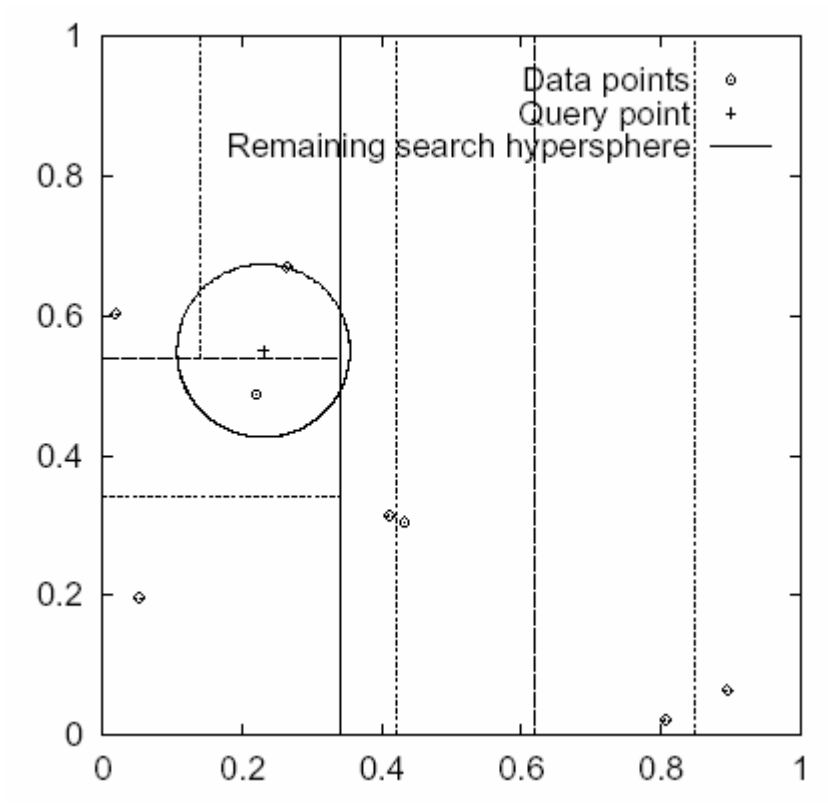
\includegraphics[width=0.8\textwidth]{figures/matching2.png}
				\caption{Feature matching using Kd tree\cite{c12}.}
			\end{figure}
		\end{columns}
	}
	\frame{
		\frametitle{Example}
		\begin{columns}
			\column[c]{.5\textwidth}
			\begin{figure}
				\centering
				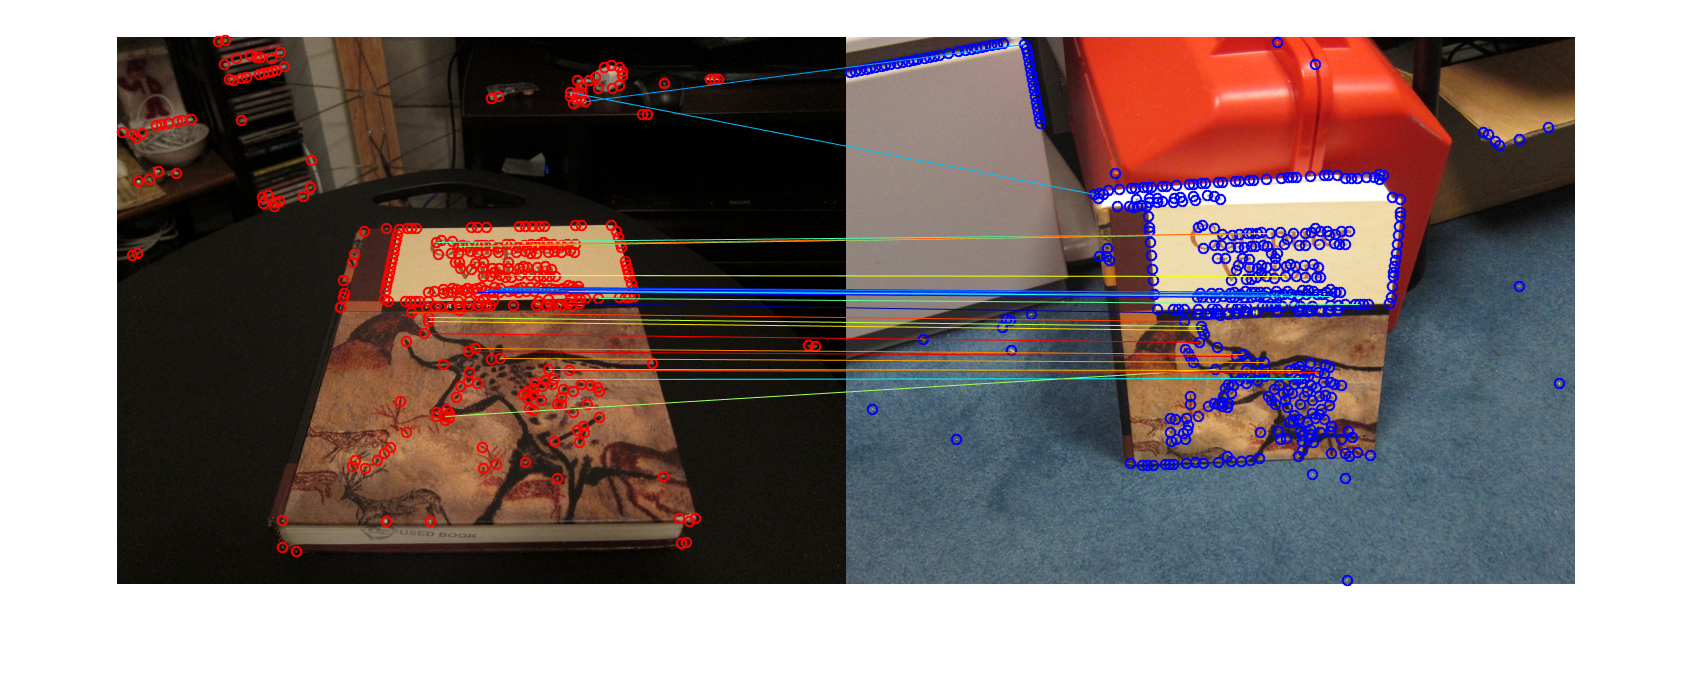
\includegraphics[width=1.\textwidth]{figures/fast.png}
				\caption{FAST$+$BRIEF matching with ratio test.}
			\end{figure}
			\column[c]{.5\textwidth}
			\begin{figure}
				\centering
				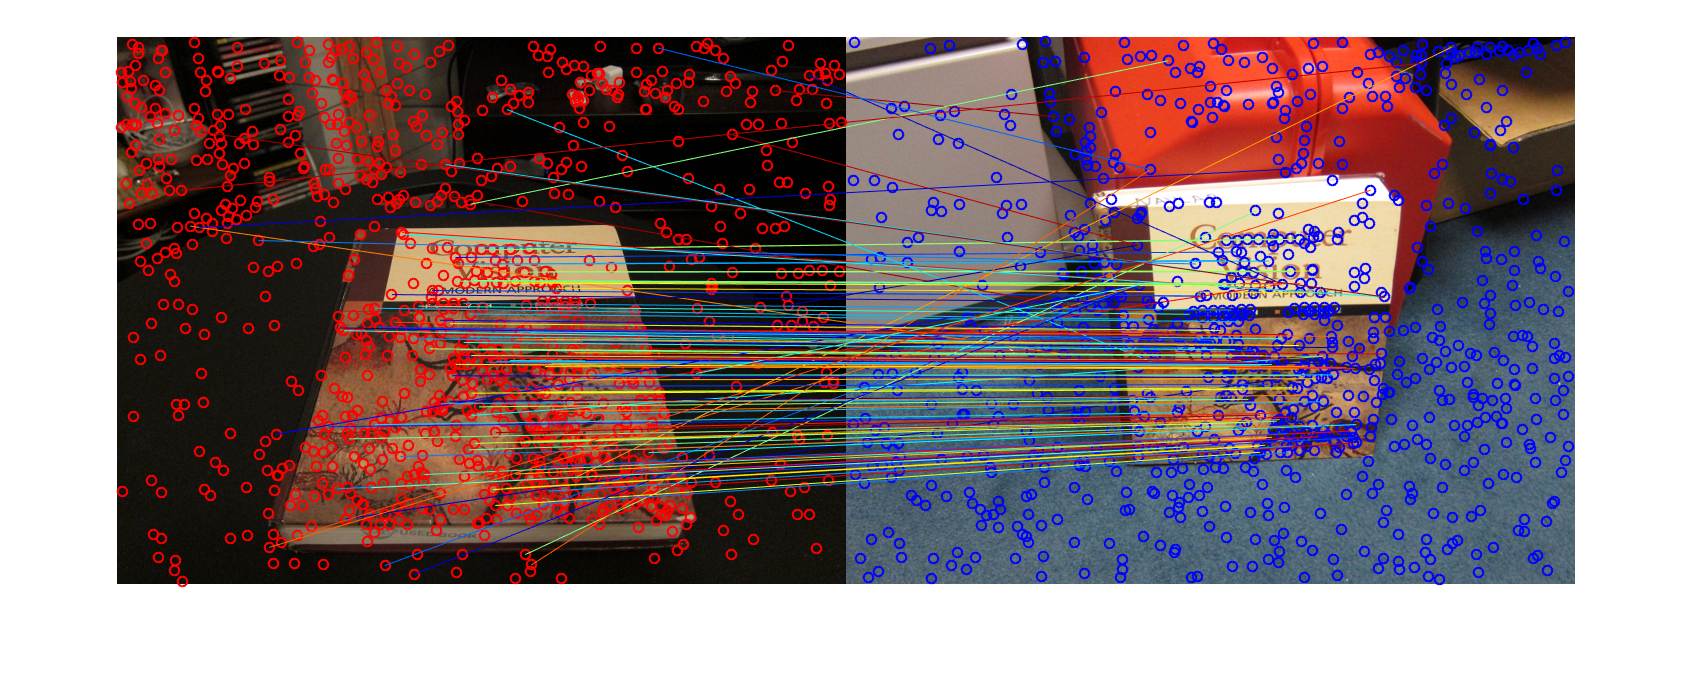
\includegraphics[width=1.\textwidth]{figures/sift.png}
				\caption{SIFT matching with ratio test.}
			\end{figure}
		\end{columns}
	}
	}
	
	\section{RANSAC}
	\subsection{Principle}
	\frame{
		\frametitle{Principle}
		\begin{columns}
			\column[c]{.5\textwidth}
			\textbf{Why need RANSAC?}
			
			Feature matching result often contains a certain amount of false matches (Outliers). Outlier will severally deteriorate the estimation result.
			
			RANSAC provides a good estimate despite the presence of a large amount outliers.
			
			\column[c]{.5\textwidth}
			\begin{figure}
				\centering
				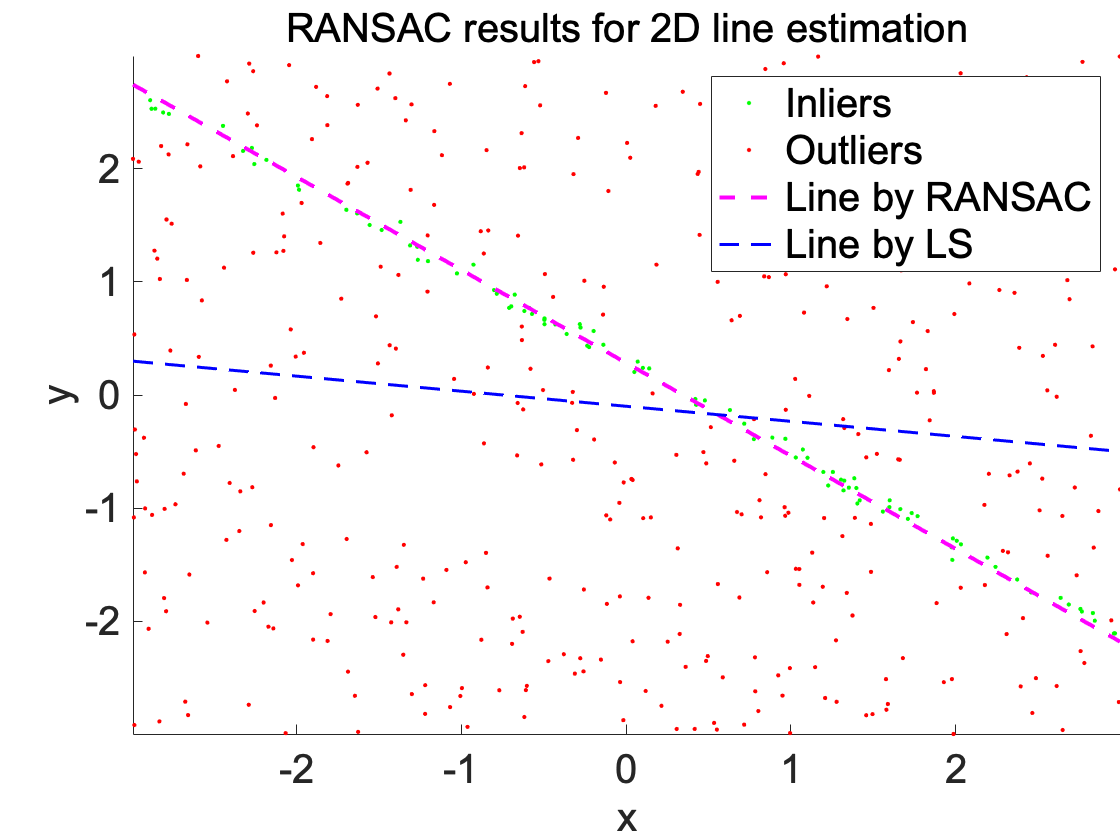
\includegraphics[width=1.\textwidth]{figures/ransac1.png}
				\caption{Line estimation results.}
			\end{figure}
		\end{columns}		
		
		
	}
	
	
	\subsection{Recent Work}	

	
		\frame{
			\frametitle{Optimization on Lie Group  for Pose Estimation}
			\only<1>{				
					\begin{figure}
					%	\includegraphics[scale=0.6]{figures/ipinmm}
						\caption{IEEE IPIN18~\cite{c2}.}
					\end{figure}
			}
			\only<2>{
				\vspace{0cm}
				\begin{columns}
					\column[c]{\textwidth}
						\centering
					%	\includegraphics[width=0.66\textwidth]{figures/res1}
				\end{columns}
			}
			\only<3>{
				\vspace{-0.2cm}
				\begin{columns}
					\column[c]{.5\textwidth}
					\begin{figure}
					%	\hspace*{-0.9cm}\includegraphics[width=7cm, height=6cm]{figures/poseest_t}
						\caption{Translation.}
					\end{figure}
					%			\vspace{-1cm}
					\column[c]{.5\textwidth}
					\begin{figure}
					%	\hspace*{-0.9cm}\includegraphics[width=7cm, height=6cm]{figures/poseest_r}	
						\caption{Rotation.}
					\end{figure}
				\end{columns}
			}	
		}
%
%\frame{
%	\frametitle{Optimization on Lie Group  for Extrinsic Calibration}
%	\only<1>{
%		\begin{block}{Result}
%			\begin{minipage}{.49\textwidth}
%				\centering
%				\includegraphics[width=1\textwidth]{figures/results/Er} 
%			\end{minipage}
%			\begin{minipage}{.49\textwidth}
%				\centering
%				\includegraphics[width=1\textwidth]{figures/results/Et}
%			\end{minipage}
%		\end{block}
%	}
%	\only<2>{
%		\begin{block}{Result}
%			\begin{columns}
%				\column[c]{.5\textwidth}
%				\centering
%				\begin{figure}
%					\includegraphics[width=0.8\textwidth]{figures/results/runtime_num} 
%				\end{figure}
%				\column[c]{.5\textwidth}
%				\centering
%				\begin{figure}
%					\includegraphics[width=0.9\textwidth]{figures/results/runtime_std}
%				\end{figure}
%			\end{columns}
%		\end{block}
%	}
%}


\frame{
	\frametitle{Trajectory Generation using SDP}
	\only<1>{
	\vspace{0cm}
	\begin{minipage}{\textwidth}
			\begin{minipage}{.325\textwidth}
				\centering

			\end{minipage}
			\begin{minipage}{.325\textwidth}
				\centering

			\end{minipage}
			\begin{minipage}{.325\textwidth}
				\centering

			\end{minipage}
	\end{minipage}
	}
	\only<2>{
		\begin{columns}
			\column{.3\textwidth}
		Alternating optimization on time allocation and polynomial coefficients:
		\begin{itemize}
			\item Relax dynamics constraints, fix $t$, optimize $\mathbf{p}$ using QP;
			\item fix $\mathbf{p}$, optimize $t$ using SDR and SDP;
		\end{itemize}
		\column{.7\textwidth}
			\centering
		\end{columns}
	}
}
	\section{Reference}
	\subsection{Ending}
	\frame{
		\centering
		{\textbf{Thank You!}
		}
	}
	
	\section{Reading Material}
	\begin{thebibliography}{00}
%		\bibitem{c3} S. {Hadfield} and K. {Lebeda} and R. {Bowden}, ``HARD-PnP: PnP Optimization Using a Hybrid Approximate Representation,`` IEEE Transactions on Pattern Analysis and Machine Intelligence, vol. 41. pp.  768-774, 2019.
	\bibitem{c1} \url{https://en.wikipedia.org/wiki/Mars_Exploration_Rover}.
	\bibitem{c2}  Chris Harris and Mike Stephens (1988). "A Combined Corner and Edge Detector". Alvey Vision Conference. 15.
	\bibitem{c3} Rosten, Edward, and Tom Drummond. "Machine learning for high-speed corner detection." European conference on computer vision. Springer, Berlin, Heidelberg, 2006.
	\bibitem{c4} Lowe, David G. "Distinctive image features from scale-invariant keypoints." International journal of computer vision 60.2 (2004): 91-110.
	\bibitem{c5} \url{https://www.uio.no/studier/emner/matnat/its/UNIK4690/v16/forelesninger/lecture_3_2_1_corner_features.pdf}.
	\bibitem{c6} Siegwart, Roland, Illah Reza Nourbakhsh, and Davide Scaramuzza. Introduction to autonomous mobile robots. MIT press, 2011.
	\bibitem{c7} J. Shi and C. Tomasi. Good Features to Track,. 9th IEEE Conference on Computer Vision and Pattern Recognition. Springer. June 1994. 
	\bibitem{c8} Calonder, Michael, et al. "BRIEF: Computing a local binary descriptor very fast." IEEE Transactions on Pattern Analysis and Machine Intelligence 34.7 (2012): 1281-1298.
	\bibitem{c9} Yi, Kwang Moo, et al. "Lift: Learned invariant feature transform." European Conference on Computer Vision. Springer, Cham, 2016.
	\bibitem{c10} DeTone, Daniel, Tomasz Malisiewicz, and Andrew Rabinovich. "Superpoint: Self-supervised interest point detection and description." Proceedings of the IEEE Conference on Computer Vision and Pattern Recognition Workshops. 2018.
	\bibitem{c11} \url{ https://www.uio.no/studier/emner/matnat/its/UNIK4690/v16/forelesninger/lecture_4_2_feature_matching.pdf}
	\bibitem{c12} \url{https://www.cs.ubc.ca/~nando/nipsfast/slides/fast04.pdf}
	\end{thebibliography}	
	
\end{document}